\section{Results and Analysis}
\label{sec:results_analysis}

We evaluate the proposed variants on six reflection-removal benchmarks, including real20, CEILNet, SIR$^2$ with ground truth, SIR$^2$ Objects, SIR$^2$ Postcard, and SIR$^2$ Wild. Table~\ref{tab:representative_methods} reports the per-dataset results of the representative methods discussed in this paper. PSNR, SSIM, and NCC are higher-is-better metrics, while LMSE measures local reconstruction error and is lower-is-better. We use the six-dataset average as the main criterion for comparing ERRNet-based methods, and treat TTA and DSRNet-S as supplementary references because they use different evaluation coverage or inference protocols.

% Required packages: booktabs, graphicx, multirow
% Cell format: PSNR / SSIM / LMSE. Higher PSNR/SSIM and lower LMSE are better.
\begin{table*}[t]
\centering
\scriptsize
\setlength{\tabcolsep}{2.8pt}
\caption{Per-dataset comparison of representative methods. Methods are ordered according to the methodological narrative. Each cell reports PSNR / SSIM / LMSE.}
\label{tab:representative_methods}
\resizebox{\textwidth}{!}{
\begin{tabular}{lccccccc}
\toprule
\multirow{2}{*}{Method}
& \multicolumn{1}{c}{real20}
& \multicolumn{1}{c}{CEILNet}
& \multicolumn{1}{c}{SIR$^2$}
& \multicolumn{1}{c}{Objects}
& \multicolumn{1}{c}{Postcard}
& \multicolumn{1}{c}{Wild}
& \multicolumn{1}{c}{Avg.} \\
& \multicolumn{7}{c}{PSNR / SSIM / LMSE} \\
\midrule
NAFNet Refiner
& 23.06 / 0.817 / 0.0201
& \textbf{30.41} / \textbf{0.961} / \textbf{0.0032}
& 23.69 / 0.889 / 0.0048
& 24.46 / 0.893 / 0.0034
& 21.51 / 0.870 / 0.0064
& \textbf{26.02} / \textbf{0.913} / \textbf{0.0048}
& \textbf{24.86} / \textbf{0.890} / \textbf{0.0071} \\
\midrule
Improved Loss
& 22.98 / 0.816 / 0.0204
& 28.80 / 0.949 / 0.0040
& 23.72 / 0.889 / 0.0047
& 24.62 / 0.896 / 0.0033
& 21.55 / 0.868 / 0.0063
& 25.80 / 0.912 / 0.0048
& 24.58 / 0.888 / 0.0072 \\
Attn Rebalanced
& \textbf{23.11} / 0.815 / 0.0210
& 28.78 / 0.954 / 0.0039
& 23.32 / 0.889 / 0.0048
& 24.53 / 0.898 / 0.0032
& 20.64 / 0.869 / 0.0059
& 25.67 / 0.904 / 0.0058
& 24.34 / 0.888 / 0.0075 \\
\midrule
Reflection Prior Branch
& 22.55 / 0.793 / 0.0262
& 27.50 / 0.937 / 0.0052
& 24.03 / 0.892 / 0.0041
& \textbf{24.94} / 0.899 / 0.0029
& 22.34 / 0.881 / 0.0042
& 25.24 / 0.899 / 0.0062
& 24.43 / 0.884 / 0.0081 \\
\midrule
Baseline + TTA$^\dagger$
& 22.45 / 0.796 / 0.0249
& 27.54 / 0.944 / 0.0046
& \textbf{24.08} / \textbf{0.895} / \textbf{0.0039}
& -- / -- / --
& -- / -- / --
& -- / -- / --
& 24.69 / 0.878 / 0.0111$^\dagger$ \\
Realistic Cascade
& 23.05 / \textbf{0.818} / \textbf{0.0197}
& 15.51 / 0.776 / 0.0174
& 23.09 / 0.880 / 0.0046
& 23.16 / 0.882 / 0.0037
& \textbf{22.82} / 0.869 / 0.0049
& 23.41 / 0.894 / 0.0057
& 21.84 / 0.853 / 0.0093 \\
\midrule
Transformer Cascade v2
& 22.69 / 0.812 / 0.0231
& 28.31 / 0.948 / 0.0041
& 23.97 / 0.894 / 0.0042
& 24.82 / \textbf{0.902} / \textbf{0.0029}
& 22.20 / \textbf{0.885} / \textbf{0.0040}
& 25.44 / 0.896 / 0.0071
& 24.57 / 0.889 / 0.0076 \\
DSRNet-S$^\ddagger$
& 20.73 / 0.765 / 0.0183
& 24.43 / 0.903 / 0.0080
& 25.31 / 0.911 / 0.0032
& 26.08 / 0.914 / 0.0025
& 24.46 / 0.909 / 0.0030
& 25.29 / 0.910 / 0.0051
& 24.38 / 0.885 / 0.0067 \\
\bottomrule
\end{tabular}}
\vspace{2pt}
\parbox{0.98\textwidth}{\footnotesize
\(\dagger\) Baseline + TTA was evaluated only on real20, CEILNet, and SIR$^2$ with ground truth; its average is over these three datasets and is not directly comparable with six-dataset averages.
\(\ddagger\) DSRNet-S is an external model evaluated with full-resolution tiled inference (tile size 512, overlap 64, AMP), reported only as a reference and excluded from boldface selection.
Bold indicates the best value among ERRNet-based methods for each dataset and metric. Higher PSNR/SSIM and lower LMSE are better.}
\end{table*}


\begin{figure*}[t]
  \centering
  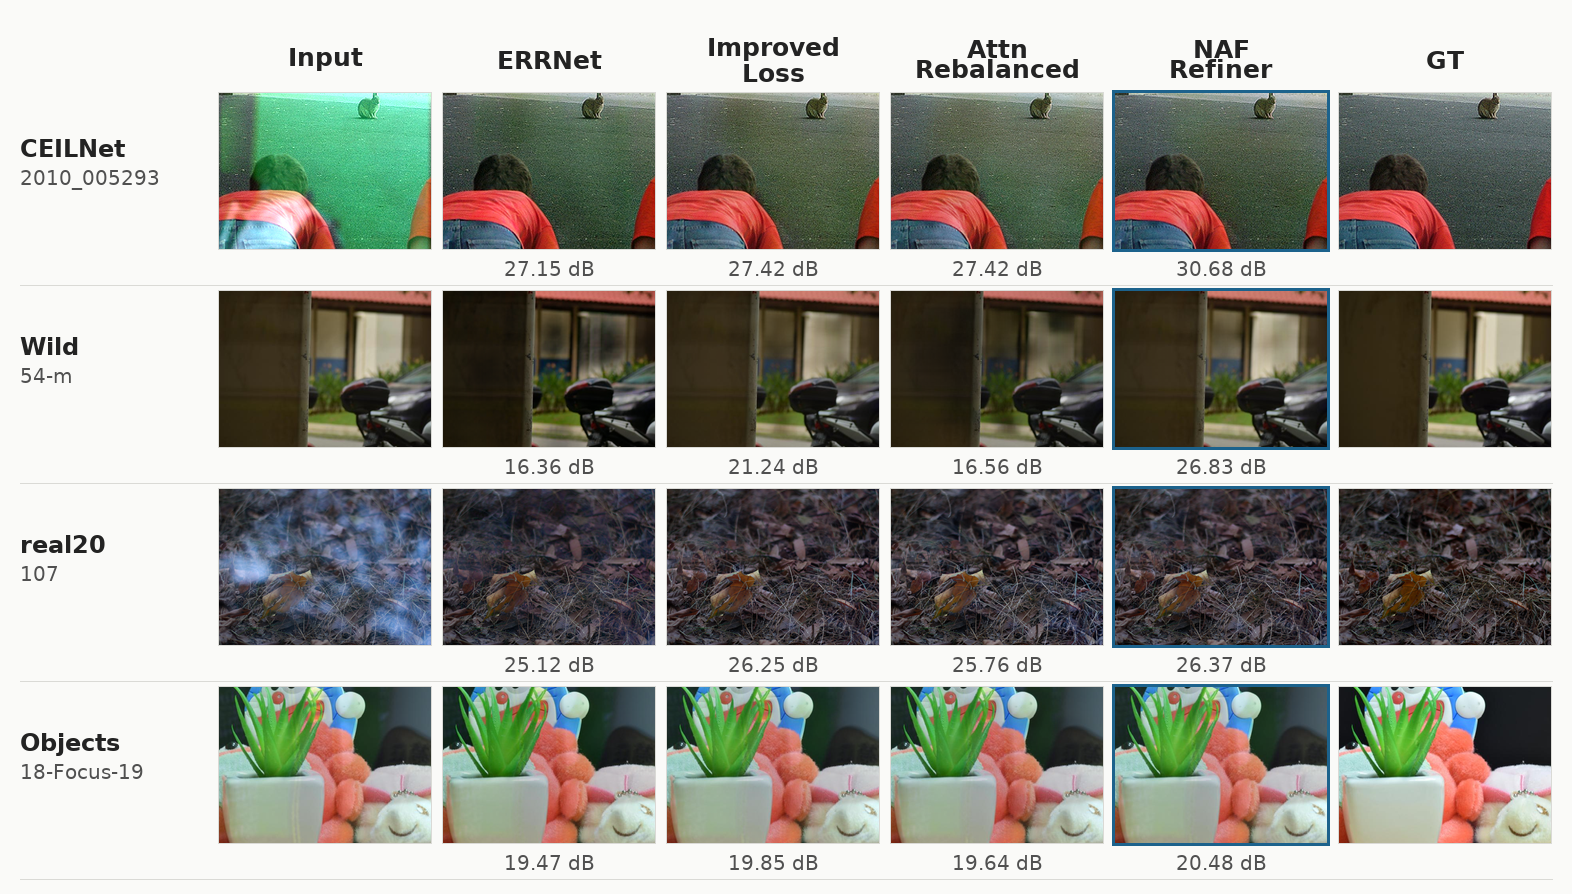
\includegraphics[width=\textwidth]{ERRNet/paper_visuals/panels/fig1_main_naf_vs_coarse.png}
  \caption{Qualitative comparison between the proposed NAFNet Refiner, the original ERRNet baseline, and two strong coarse-model variants. The examples cover synthetic, wild, real, and object-scene data. The blue boxes indicate the final NAFNet Refiner.}
  \label{fig:qual_main}
\end{figure*}

\begin{figure*}[t]
  \centering
  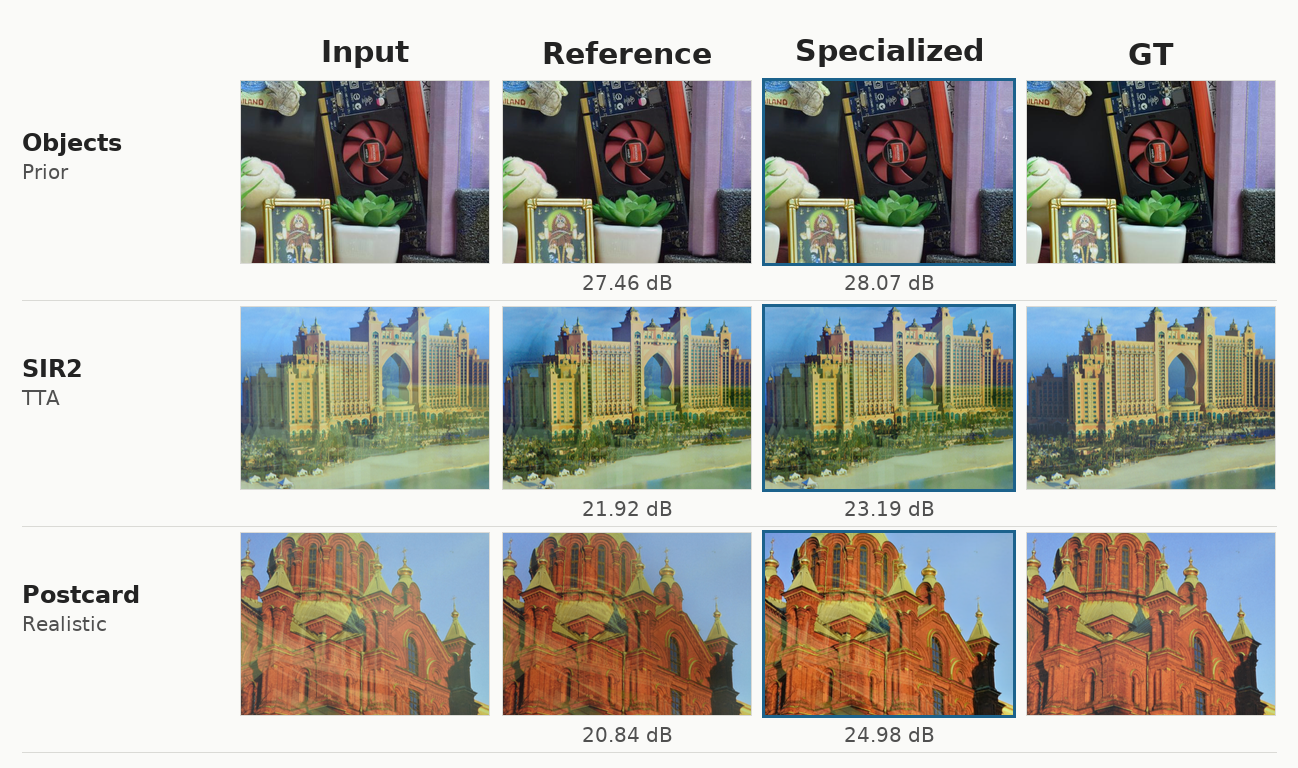
\includegraphics[width=0.92\textwidth]{ERRNet/paper_visuals/panels/fig2_specialized_methods.png}
  \caption{Qualitative examples of dataset-specialized methods. The prior branch, test-time augmentation, and realistic cascade address different failure modes: spatially localized reflection, inference instability, and realistic reflection statistics.}
  \label{fig:qual_specialized}
\end{figure*}

\begin{figure*}[t]
  \centering
  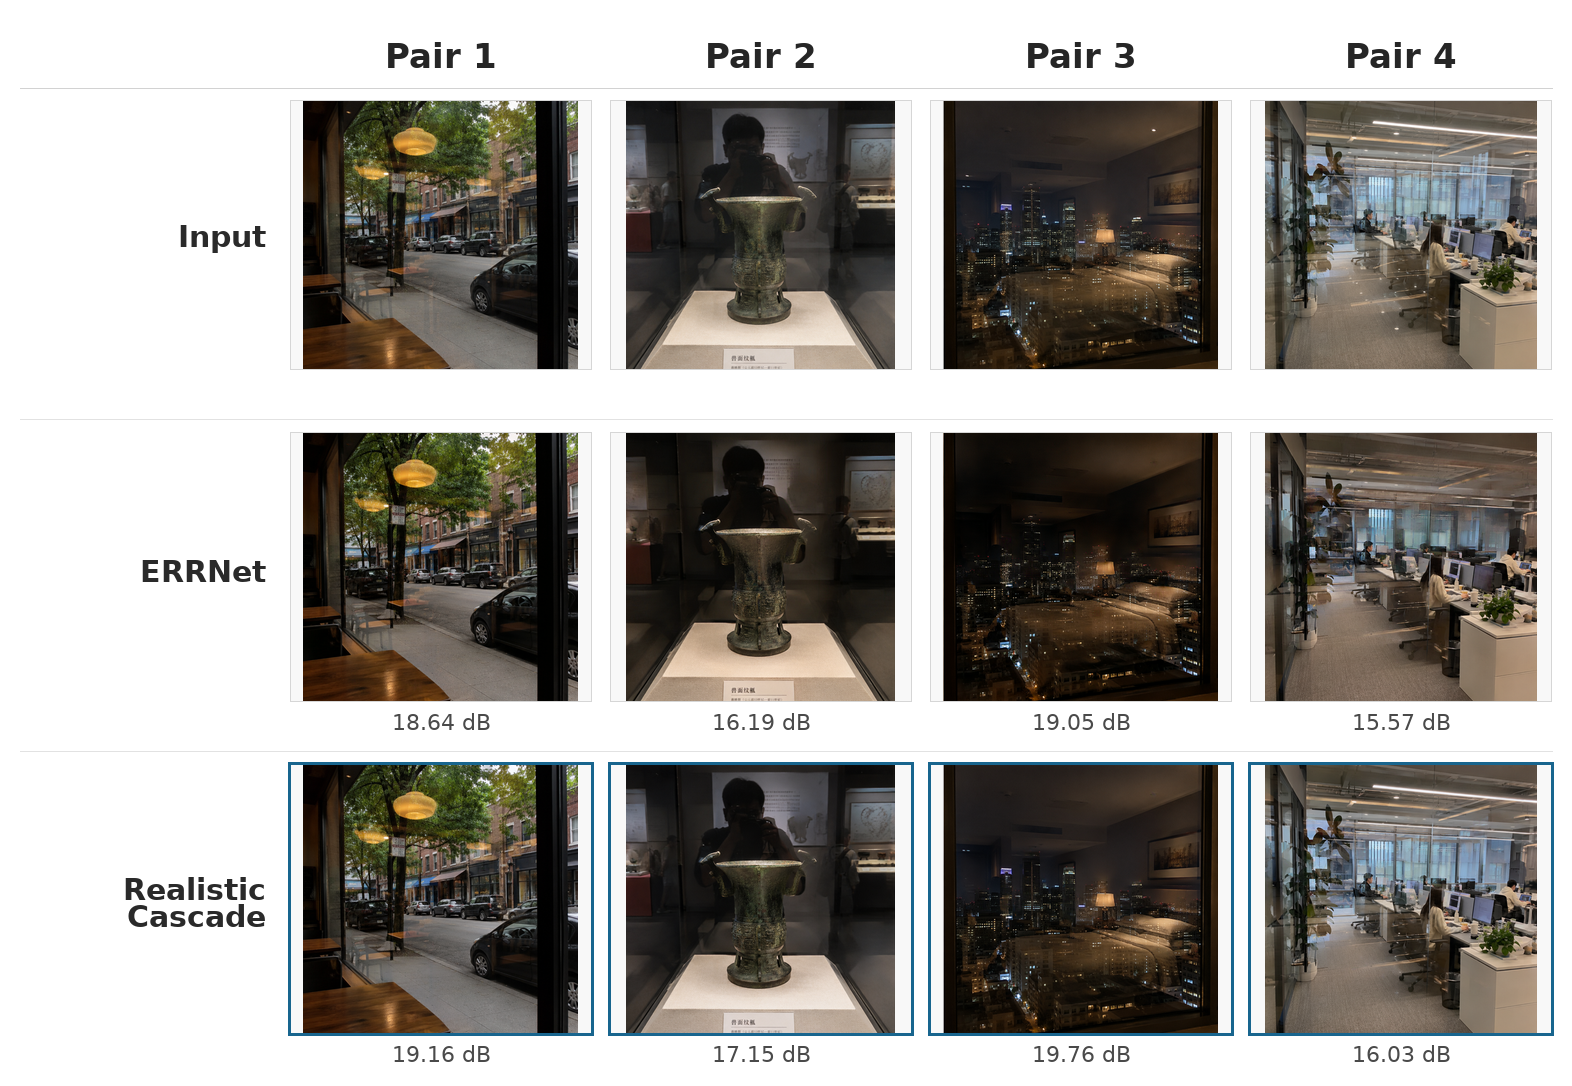
\includegraphics[width=\textwidth]{ERRNet/paper_visuals/panels/fig3_reflection_pairs_tight_horizontal_nogt.png}
  \caption{Qualitative comparison on the tight reflection-pair set. Realistic Cascade is the best average method on this set and is compared with the original ERRNet output and the input image. PSNR values are reported below the restored outputs.}
  \label{fig:tight_pairs}
\end{figure*}

\subsection{Overall Quantitative Comparison}

The most important quantitative observation is that the strongest result is obtained by a conservative coarse-to-fine design rather than by replacing ERRNet with a substantially larger or more global architecture. The NAFNet Refiner achieves the best six-dataset average among ERRNet-based methods, reaching 24.86 dB PSNR, 0.890 SSIM, and 0.0071 LMSE. Compared with the original ERRNet baseline, it improves the average PSNR by 0.45 dB and reduces the average LMSE from 0.0080 to 0.0071. Compared with the Improved Loss coarse model, which is already a strong baseline, the refiner still brings a further gain of 0.28 dB in average PSNR. This indicates that the second-stage refinement does not merely benefit from a stronger first-stage model; it learns a complementary correction that the coarse ERRNet output does not capture.

The gains are not uniformly distributed across datasets, and this distribution is informative. On CEILNet, NAFNet Refiner improves from 27.26 dB for ERRNet and 28.80 dB for Improved Loss to 30.41 dB. On SIR$^2$ Wild, it improves from 25.45 dB for ERRNet and 25.80 dB for Improved Loss to 26.02 dB. These two datasets are precisely where the coarse model tends to leave low-frequency color residuals or thin reflection edges. In contrast, on SIR$^2$ Objects and SIR$^2$ Postcard, the best single-dataset results are obtained by Reflection Prior Branch and Realistic Cascade, respectively. This shows that the final NAFNet Refiner is the best general-purpose model, while other variants capture useful dataset-specific biases.

The comparison also clarifies why our final method uses residual refinement instead of direct architectural substitution. The single Transformer variant performs poorly, and Transformer Cascade v2 is competitive but does not exceed the NAFNet Refiner in average PSNR or LMSE. This suggests that global attention alone is not the bottleneck of the task. Reflection removal is highly sensitive to local color, edge, and texture fidelity; an unconstrained global module can easily disturb the already plausible transmission layer. In contrast, the NAFNet Refiner starts from a strong coarse estimate and predicts only a bounded residual correction, which makes the optimization target more local and better conditioned.

\subsection{Qualitative Effect of Coarse-to-Fine Refinement}

Figure~\ref{fig:qual_main} provides qualitative evidence for the above interpretation. Across the four representative examples, ERRNet removes part of the reflection but often leaves one of three artifacts: residual color cast, over-smoothed structure, or incorrect local contrast. The Improved Loss and Attn Rebalanced variants improve the coarse prediction by changing the training objective, but their corrections remain limited by the one-stage ERRNet representation. The NAFNet Refiner consistently produces a cleaner and more natural transmission layer.

In the CEILNet example, the input contains a strong green reflection component. ERRNet and the two coarse-model variants suppress the dominant reflection, but a noticeable chromatic bias remains and the recovered scene still appears contaminated. The NAFNet Refiner removes more of this residual cast while preserving the red clothing and background texture, yielding a result much closer to the ground truth. This is consistent with the design of the refiner input, which concatenates the original image, the coarse output, and the residual image. The residual channel explicitly exposes the part of the observation that is not explained by the coarse transmission estimate, allowing the refiner to focus on remaining reflection evidence instead of relearning the whole mapping.

The Wild example further illustrates why residual refinement is useful. The original ERRNet output remains blurred and low-contrast, and Attn Rebalanced does not fully correct this failure. Improved Loss improves the scene, but the NAFNet Refiner produces a substantially sharper and cleaner output, as reflected by the increase to 26.83 dB in the selected example. This behavior supports our hypothesis that a strong coarse model recovers the global scene layout, while the second stage mainly restores local contrast and removes reflection-layer remnants. Since the NAF branch is initialized to predict zero residual, it begins from the coarse output and learns corrections only where the training signal consistently indicates improvement. This conservative initialization is crucial: it reduces the risk that the second stage damages already well-recovered regions.

In the real20 and Objects examples, the improvement is more subtle but still important. On real20, the remaining blue reflection veil is weakened without destroying the fine texture of the leaves and background. On Objects, the final output better separates the foreground objects from the reflection-contaminated background and improves color consistency. These cases show that the NAFNet Refiner is not simply increasing image sharpness. Instead, it selectively adjusts local residuals while keeping the transmitted scene structurally stable. This explains why the method improves the average LMSE as well as PSNR: local reconstruction errors are reduced rather than only global intensity statistics being corrected.

\subsection{Why Specialized Variants Help on Specific Datasets}

Although the NAFNet Refiner is the strongest average method, Figure~\ref{fig:qual_specialized} shows that several non-final variants provide meaningful evidence for our design choices. Each specialized method corresponds to a different reflection-removal difficulty.

The Reflection Prior Branch is most useful when the reflection is spatially localized. In the Objects example, the prior-based output improves over the reference from 27.46 dB to 28.07 dB. The key difference is not a global change in color or contrast, but a more spatially controlled correction. The prior branch predicts a reflection-related mask from the input, coarse output, residual magnitude, and fixed high-frequency responses. This mask gates the residual update, encouraging the model to modify regions that are likely to contain reflection while preserving regions that already resemble the clean transmission layer. The visual result supports this design: the specialized output corrects local contamination without introducing unnecessary changes across the whole image. This also explains the quantitative behavior in Table~\ref{tab:representative_methods}, where Reflection Prior Branch achieves the best Objects PSNR among ERRNet-based methods but is weaker on datasets where the reflection is diffuse or the pseudo-mask is less reliable.

The TTA example shows a different kind of improvement. Baseline + TTA increases the selected SIR$^2$ example from 21.92 dB to 23.19 dB. Since TTA does not change model parameters, the gain should be interpreted as a reduction of inference variance. Low-level restoration networks are expected to be approximately equivariant to horizontal and vertical flips, but finite training data and asymmetric reflection patterns make the actual predictions direction-dependent. Averaging flipped predictions suppresses unstable artifacts and improves color consistency. This explains why TTA is helpful on some SIR$^2$ cases and CEILNet, while it is not adopted as the universal default: for real reflections whose appearance is strongly tied to physical direction, averaging multiple transformed predictions can also attenuate valid details.

The Postcard example demonstrates the value of Realistic Cascade. In this case, the specialized method improves from 20.84 dB for the reference output to 24.98 dB. Postcard images often contain strong texture, saturated color, and reflection patterns that are tightly mixed with scene structure. A model trained only on simpler synthetic mixtures may either leave visible ghosting or over-suppress real texture. Realistic Cascade addresses this by combining more realistic online synthesis with a cascade residual network. The realistic synthesis introduces spatially varying reflection strength, ghost shifts, color gain, gamma-domain blending, noise, and compression artifacts, making the training distribution closer to real glass reflections. The cascade structure then refines the coarse output instead of predicting the clean image in one step. The visual result confirms this mechanism: the specialized output removes more overlay-like reflection while preserving the architectural details of the building.

These observations are important because they prevent an overly simplistic conclusion. The best average model is not the only useful model. Rather, the experiments identify three complementary principles: residual refinement improves general restoration quality, spatial priors improve localized reflection handling, and realistic degradation modeling improves robustness to complex real-world reflection statistics.

\subsection{Comparison with ERRNet Beyond Standard Metrics}

Figure~\ref{fig:tight_pairs} focuses on the tight reflection-pair set and compares Realistic Cascade with the original ERRNet without displaying the ground truth. This figure is useful because it emphasizes perceptual behavior in realistic glass-reflection scenes rather than only benchmark-aligned numerical performance. On this set, Realistic Cascade ranks first with 17.90 dB average PSNR, while the original ERRNet obtains 17.41 dB. More importantly, the visual differences reveal how the algorithmic design changes the output.

In Pair 1, ERRNet darkens the scene and leaves a less natural balance between the indoor reflection and outdoor street. Realistic Cascade better preserves the outdoor structure and local brightness while reducing the reflected layer. In Pair 2, the museum glass reflection is difficult because the reflected human silhouette overlaps the object of interest. ERRNet suppresses part of the reflection but also compresses the overall tone. Realistic Cascade keeps the vessel more visible and produces a more stable background-object separation. In Pair 3, the night scene contains dense city lights and indoor reflections. ERRNet tends to produce a darker output with compressed local detail; Realistic Cascade keeps more visible structure in the city lights while reducing the reflected interior layer. In Pair 4, the office scene contains large-area transparent glass reflections. The cascade output better preserves the spatial layout of the office and avoids excessive darkening.

These improvements directly reflect the design of Realistic Cascade. Realistic synthesis exposes the model to reflection phenomena that standard synthetic mixtures do not cover, such as shifted ghost images, nonuniform reflection intensity, and camera-processing artifacts. The cascade refiner then corrects the coarse output progressively, which is better suited to real glass scenes where reflection and transmission are not separable by a single global intensity rule. Therefore, even though Realistic Cascade is not the best six-dataset method because it mismatches CEILNet-style synthetic data, it provides strong evidence that realistic data modeling improves perceptual behavior on real reflection pairs.

\subsection{Failure Modes and Implications}

The results also reveal several limitations. First, stronger refinement can over-correct. NAFNet Refiner is best on average, but it is not the best on SIR$^2$ Objects, SIR$^2$ Postcard, or SIR$^2$ with ground truth. These datasets include cases where the baseline ERRNet already preserves the transmission layer well, or where the reflection statistics differ from the dominant training distribution. In such cases, an ungated residual refiner may introduce unnecessary corrections. This explains why the Reflection Prior Branch remains valuable despite its lower average score: it provides a mechanism for protecting non-reflection regions.

Second, realistic synthesis improves real and postcard-like cases but can hurt synthetic benchmark generalization. Realistic Cascade performs well on the tight reflection-pair set and obtains the best ERRNet-based Postcard PSNR in Table~\ref{tab:representative_methods}, but its CEILNet result is very low. This indicates a distribution conflict between the realistic degradation prior and the CEILNet test distribution. A practical system should therefore avoid using a single synthesis policy for all datasets. A better future direction is to combine realistic synthesis with a confidence-based selector or a gated refiner that can decide when to trust the realistic cascade.

Third, adding model capacity or global context is not sufficient. Transformer Cascade v2 has strong SSIM on Objects and Postcard, but the plain Transformer variant fails substantially. This supports the broader conclusion that reflection removal benefits from constrained correction rather than unconstrained reconstruction. The most reliable improvements come from preserving a strong coarse solution and learning where and how to modify it.

\subsection{Summary}

Overall, the experiments demonstrate that our method family improves over the original ERRNet in both numerical performance and perceptual restoration quality. The main result, NAFNet Refiner, validates the central idea of using a strong ERRNet coarse model followed by conservative residual refinement. It improves average PSNR, SSIM, and LMSE, and visually reduces residual color cast, reflection veil, and local texture errors. The specialized variants further explain which design components matter under different conditions: the prior branch improves spatially localized correction, TTA improves prediction stability, and Realistic Cascade improves robustness to realistic glass-reflection statistics. Thus, the contribution is not only a higher-scoring model, but a clearer decomposition of single-image reflection removal into coarse transmission recovery, residual correction, spatial control, and distribution-aware refinement.
